\newacronym{www}{WWW}{World Wide Web}
\newacronym{w3c}{W3C}{World Wide Web Consortium}
\newacronym{nlp}{NLP}{Natural Language Processing}
\newacronym{rdf}{RDF}{Resource Description Framework}
\newacronym{xml}{XML}{Extended Markup Language}
\newacronym{r2rml}{R2RML}{RDB to RDF Mapping Language}
\newacronym{sca}{SCA}{Semantic Content Authoring}
\newacronym{sql}{SQL}{Structured Query Language}
\newacronym{sparql}{SPARQL}{Semantic Protocol and RDF Query Language}
\newacronym{ie}{IE}{Information Extraction}
\newacronym{ui}{UI}{User Interface}

\section{Crowdsourcing in the Semantic Web}\label{sec:state_of_the_art_crowdsourcing_and_the_semantic_web}
This section starts by briefly introducing the Semantic Web and the driving ideas in it's early stages. The central part of this section is dedicated to discussing the interplay between the Semantic Web and Crowdsourcing by the \textit{Linked~Data~Life-Cycle}. 

The \gls{www} was probably one of the most influential and World changing innovation, allowing users to exchange documents without caring about the details of how they are processed or stored. The Semantic Web adds another layer on-top, enabling the use of references to real-world objects without concerning about the underlying documents in which these things are described. To that sense, the Semantic Web can be seen as an extension of the \gls{www}. It provides the means to process data in machine-readable formats, linking related properties to globally accessible schemas and offering a wide range of data interfaces~\cite{hendler2010}.
The adoption of Semantic Web technologies is still ongoing, many applications were developed that exploit these principles, but its full potential is just starting to be explored. This holds in particular because many tasks can not be fully automated or it would be too costly. Crowdsourcing, on the other hand, facilitates distribution of tasks to a large number of contributors in a scalable and affordable way. In the remainder of this section we analyse, how Crowdsourcing can promote the adoption of Semantic Web technologies. 

\subsection{The Linked Data Life-Cycle}
Over the years many tools and practices were developed that cover the full life cycle of weaving the Semantic Web. The stages of the Linked Data Life-Cycle are illustrated in~\hyperref[fig:linked_data_life_cycle]{Figure~\ref*{fig:linked_data_life_cycle}}. It shows the overall process of Linked Data management, starting from adding links and ending in manual authoring. 
\begin{figure}
	 \centering
	 
\includegraphics[width=0.75\textwidth]{drawio/Linked_Data_Life_Cycle}
	 \caption{The Linked Data Life-Cycle~(consolidated from~\cite{auer2011, auer2012, siorpaes2008})}\label{fig:linked_data_life_cycle}
\end{figure}  
Although the life cycle for semantic content starts with conceptual modelling~(e.g. mapping unstructured data to structured or semi-structured formalisms), this is not always the case, especially if existing linked data should be managed as well. In that case, the first stage~(Extraction) can be omitted. Likewise, the stages of the life cycle do not exist in isolation of each other or are passed in strict order, instead they are mutually complementary. Consequently, the examples that were given in each stage may also be relevant for other stages~\cite{simperl2013}. 

\paragraph{Extraction} When starting from scratch, data encoded in different formalisms need to be mapped to the semantic data model to facilitate semantic processing. 
There exist several approaches for the extraction process. When considering unstructured sources, text in particular, \emph{\gls{nlp}} as well as \emph{\gls{ie}} techniques have been successfully applied to gather relevant information. Three sub-disciples of \gls{nlp} have emerged: \emph{Named~Entity~Recognition} for discovering entity instances, \emph{Keyword/Keyphrase~Extraction} for identifying common topics and \emph{Relationship~Extraction} for linking entities to keywords. For structured data such as \gls{xml} there exist a number of approaches. For example, the \gls{w3c} published the recommendation \gls{r2rml}\footnote{\url{http://www.w3.org/TR/r2rml/} accessed 2018/08/06} which describes a common notation for mapping relational tables, views and queries to \gls{rdf}. 

Probably the most popular example of a community created/maintained knowledge base is Wikipedia\footnote{\url{https://www.wikipedia.org/} accessed 2018/08/06}. A little known fact is that its central platform for data management is Wikidata\footnote{\url{https://www.wikidata.org/wiki/Wikidata:Main_Page} accessed 2018/08/06}, a knowledge base containing millions of entities, labels and descriptions. For example, the page for Tim~Berners-Lee, a computer scientist and the \guillemotright author\guillemotleft~of the \gls{www}, contains properties in different languages~(excerpt shown in~\hyperref[fig:wikidata_tim_berners_lee_lang]{Figure~\ref*{fig:wikidata_tim_berners_lee_lang}}) as well as statements of him as a person~(excerpt shown in~\hyperref[fig:wikidata_tim_berners_lee_stat]{Figure~\ref*{fig:wikidata_tim_berners_lee_stat}}). 
\begin{figure}
	 \centering
	 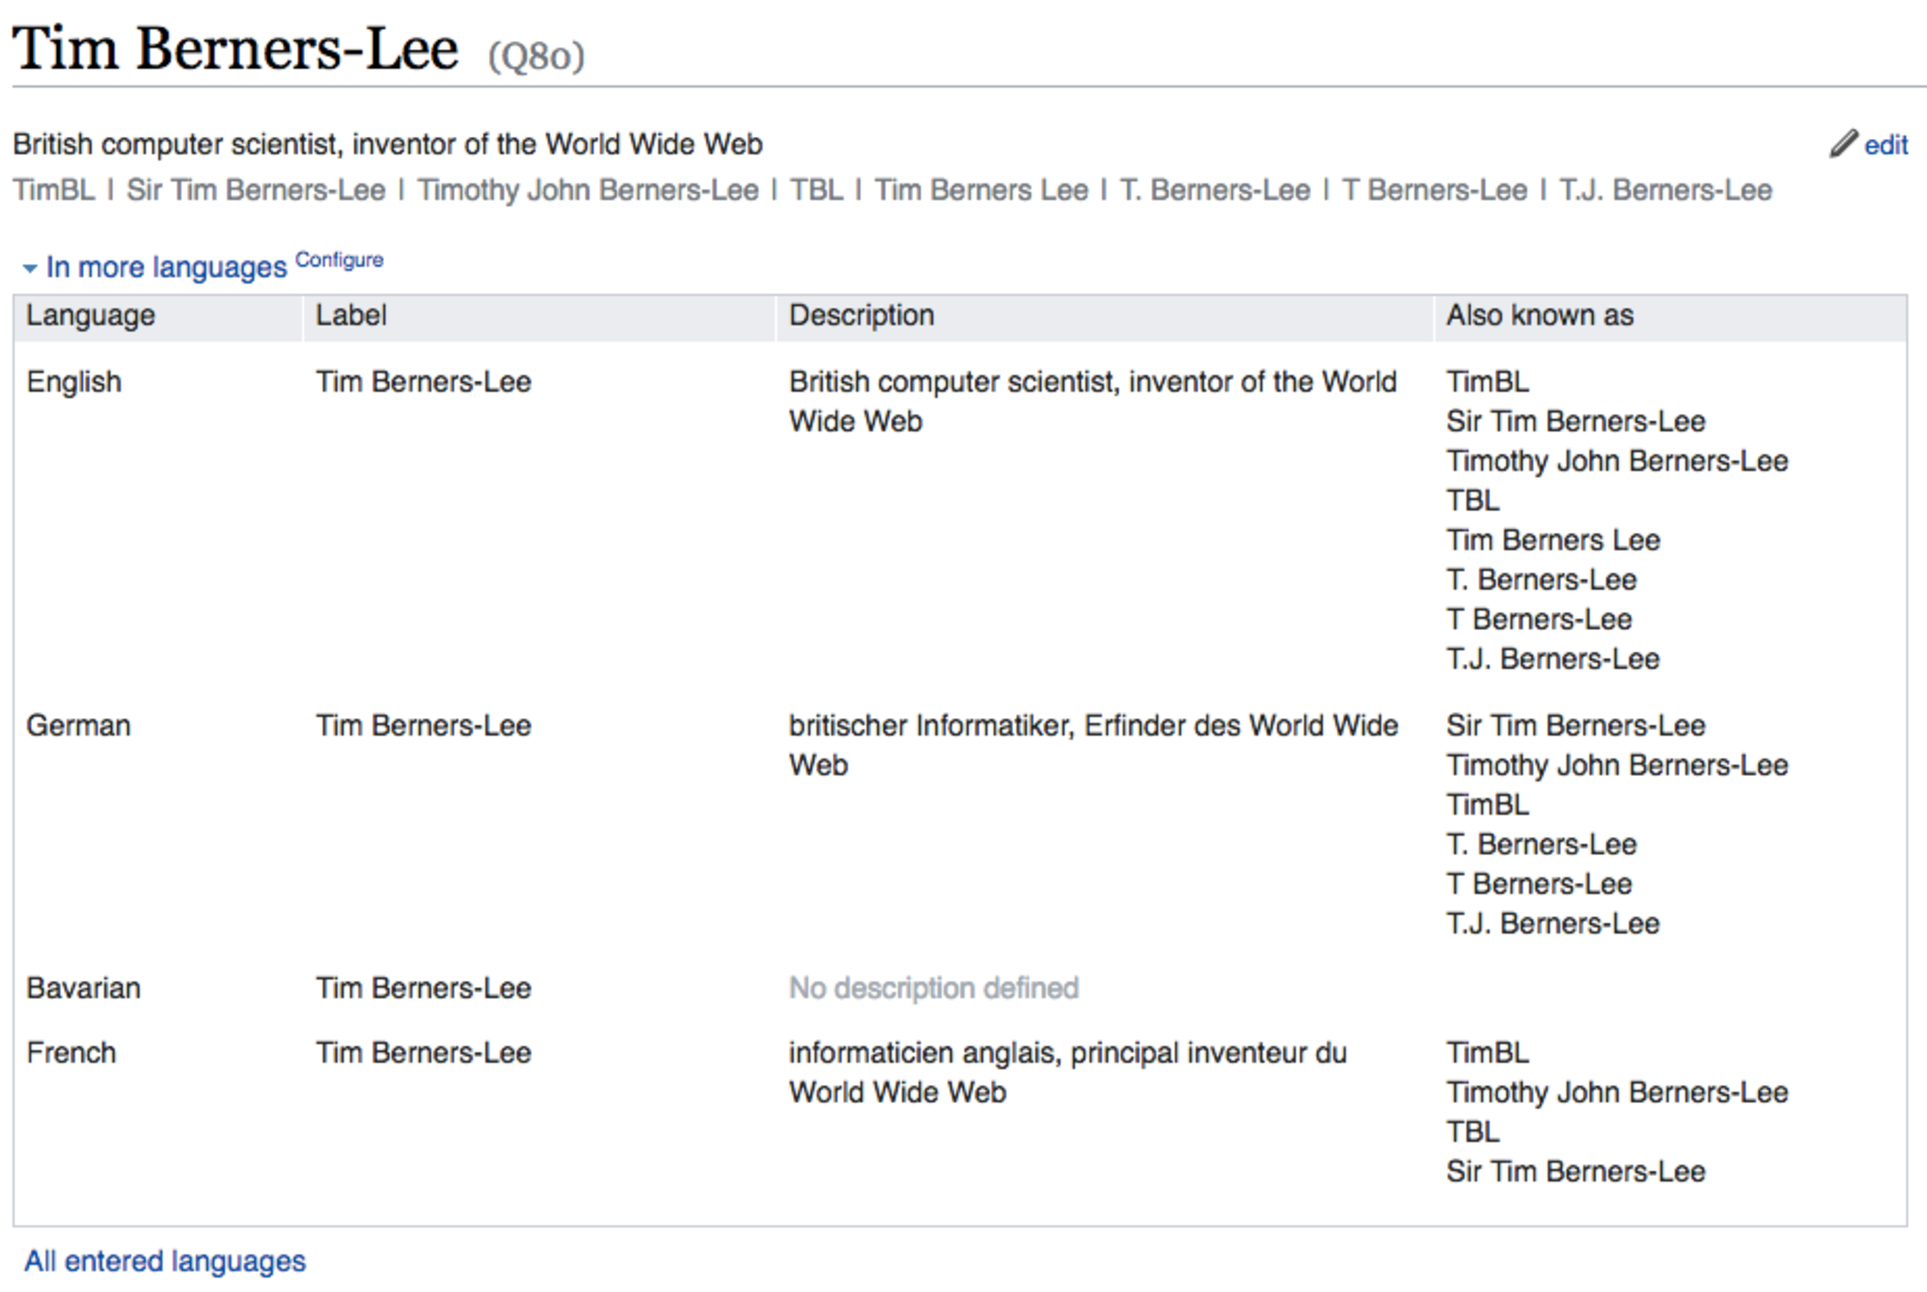
\includegraphics[width=0.75\textwidth]{graphics/wikidata_tim_berners_lee_lang}
	 \caption{Excerpt of a Wikidata page showing language properties of Tim~Berners-Lee}\label{fig:wikidata_tim_berners_lee_lang}
\end{figure}
\begin{figure}
	 \centering
	 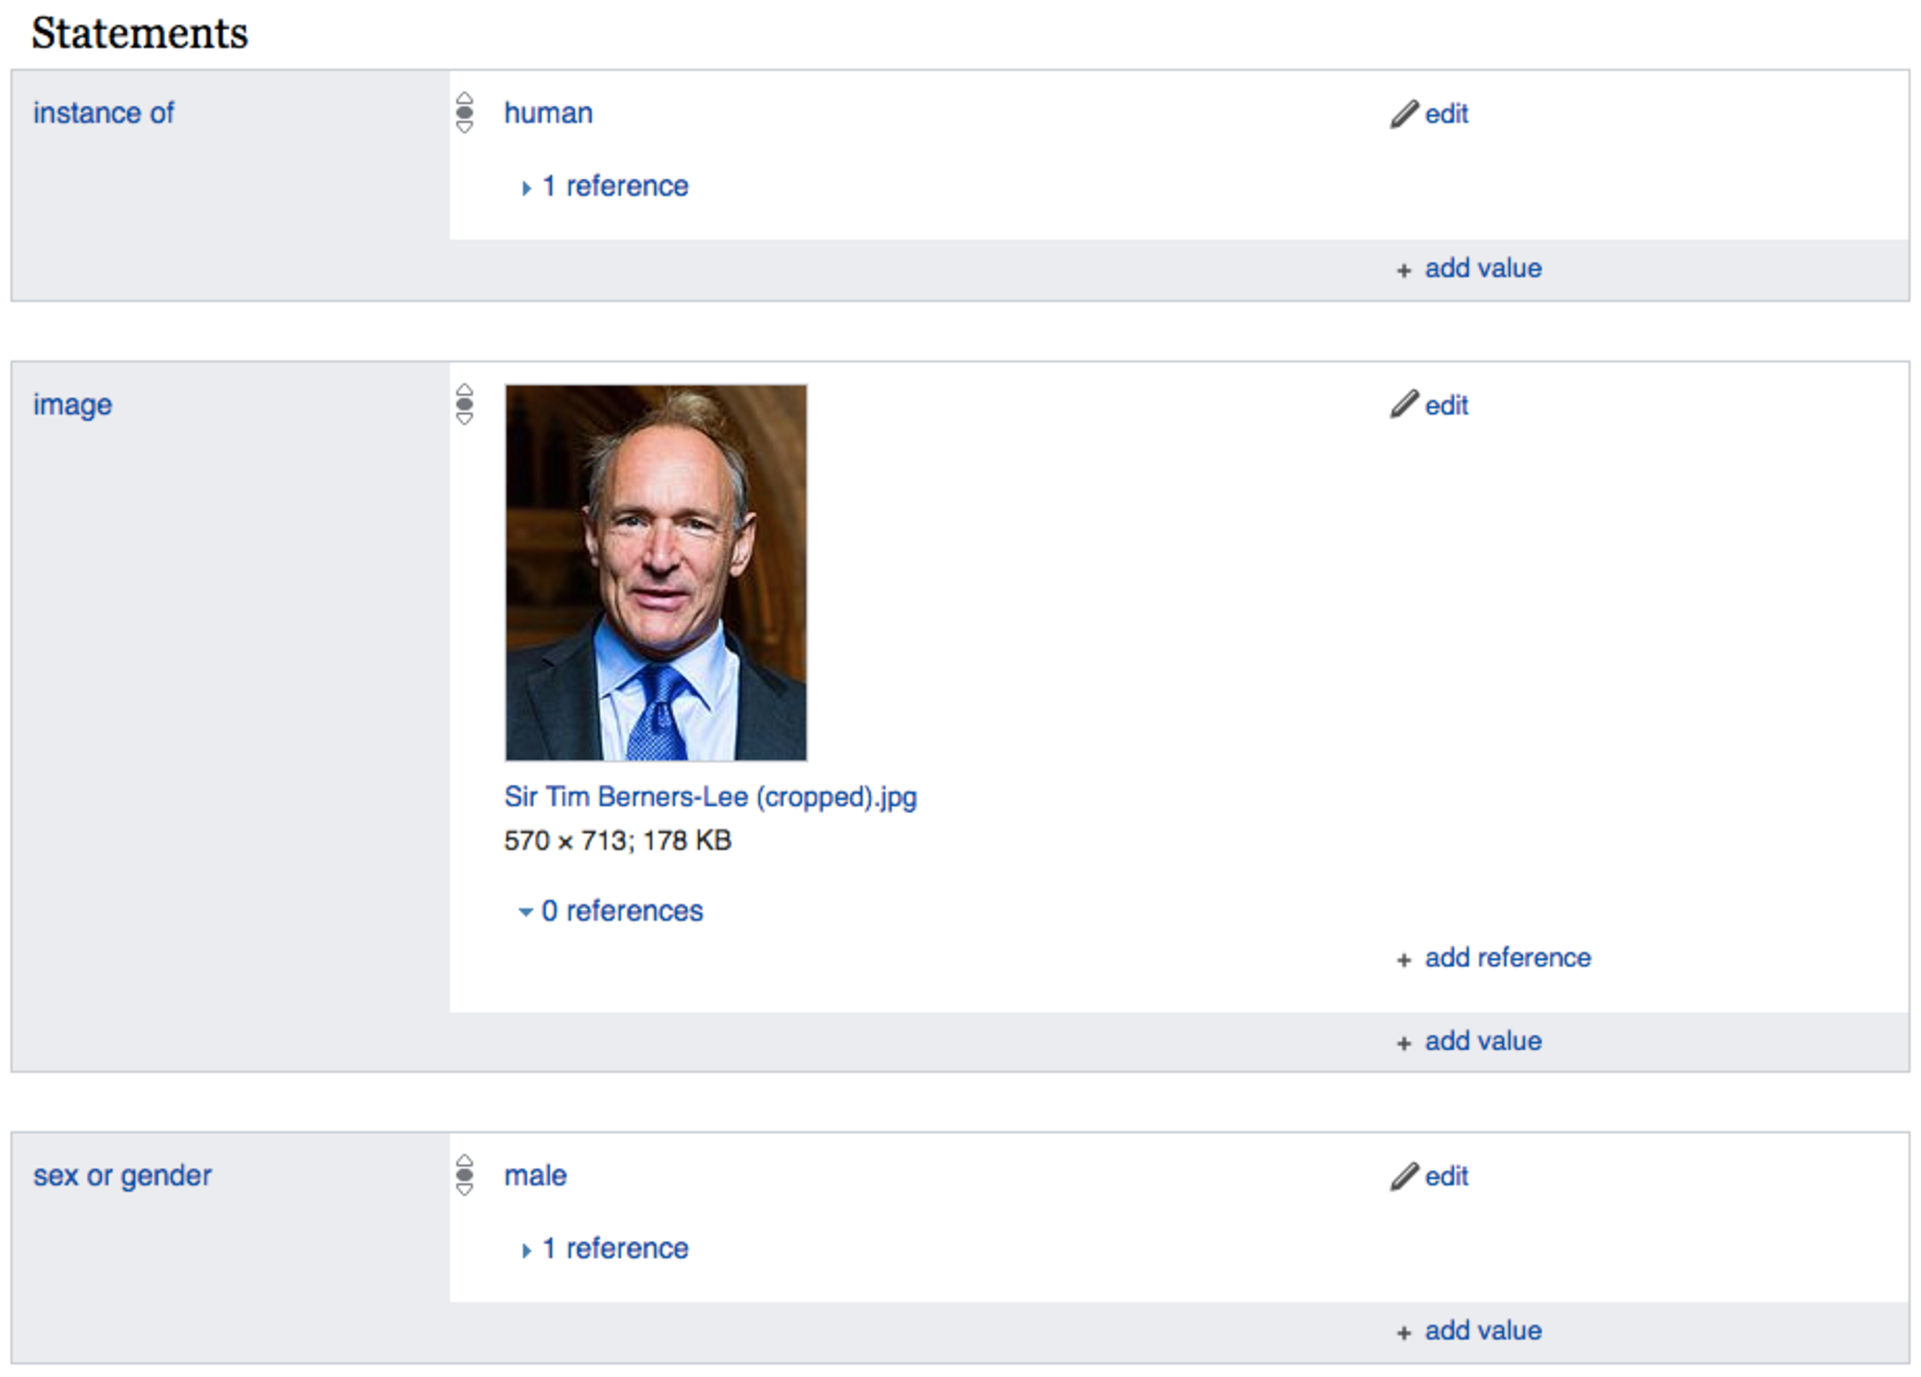
\includegraphics[width=0.75\textwidth]{graphics/wikidata_tim_berners_lee_stat}
	 \caption{Excerpt of a Wikidata page showing statements of Tim~Berners-Lee}\label{fig:wikidata_tim_berners_lee_stat}
\end{figure}
Every page has a unique identifier~(e.g. \texttt{Q80}), a label~(e.g. \texttt{Tim~Berners-Lee}), a brief description~(e.g. \texttt{British computer scientist, inventor of the \gls{www}}), a list of aliases~(e.g. \texttt{TimBLSir, Tim Berners-LeeTimothy, John Berners-Lee, \ldots}), a list of statements~(e.g. \texttt{instanceof, image, \ldots}) and some links. 
It is obvious that these data would perfectly fit into the Linked Data model~\cite{erxleben2014}.
Wikidata content is also available in \gls{rdf} which is accessible at \url{http://tools.wmflabs.org/wikidata-exports/rdf/}. Unfortunately, this data is provided via dump files\footnote{\url{https://tools.wmflabs.org/wikidata-exports/rdf/exports.html} accessed 2018/08/06} only.

\paragraph{Data Storage and Indexing} 
Up to this stage, the data was already mapped to the \gls{rdf} data model but needs to be stored and indexed efficiently. Researchers have put a lot
of effort into this field because efficient storage and indexing mechanisms are fundamental for the adoption of Linked Data. Due to efficient querying and storage capabilities of relational databases resulting from decades of research in this area, it makes sense to adopt these approaches for Linked Data as well~\cite{abadi2007}. However, to support storing very large quantities of data there exist custom solutions too~\cite{broekstra2002}. 

Targeting Linked Data indexing, various approaches and principles have been applied successfully. The common aspects of all approaches is their focus on \emph{Data Compression} and \emph{Data Pruning}~\cite{svoboda2011}. Whereas the basic idea of Data Compression is to minimise the footprint of the index, Data Pruning is a technique for avoiding unnecessary data processing. 

\paragraph{Data Revision and Authoring} In this stage users are given the opportunity to create new or modify existing semantic information. 
This is called \textit{\gls{sca}} which is defined in the literature as~\textit{"a tool-supported
manual composition process aiming at the creation of semantic documents."}~\cite{khalili2013} More generally speaking, \gls{sca} is actually embedded in a broader ecosystem for semantic content authoring as shown in~\hyperref[fig:authoring_semantic_ecosystem]{Figure~\ref*{fig:authoring_semantic_ecosystem}}. 
\begin{figure}
	 \centering
	 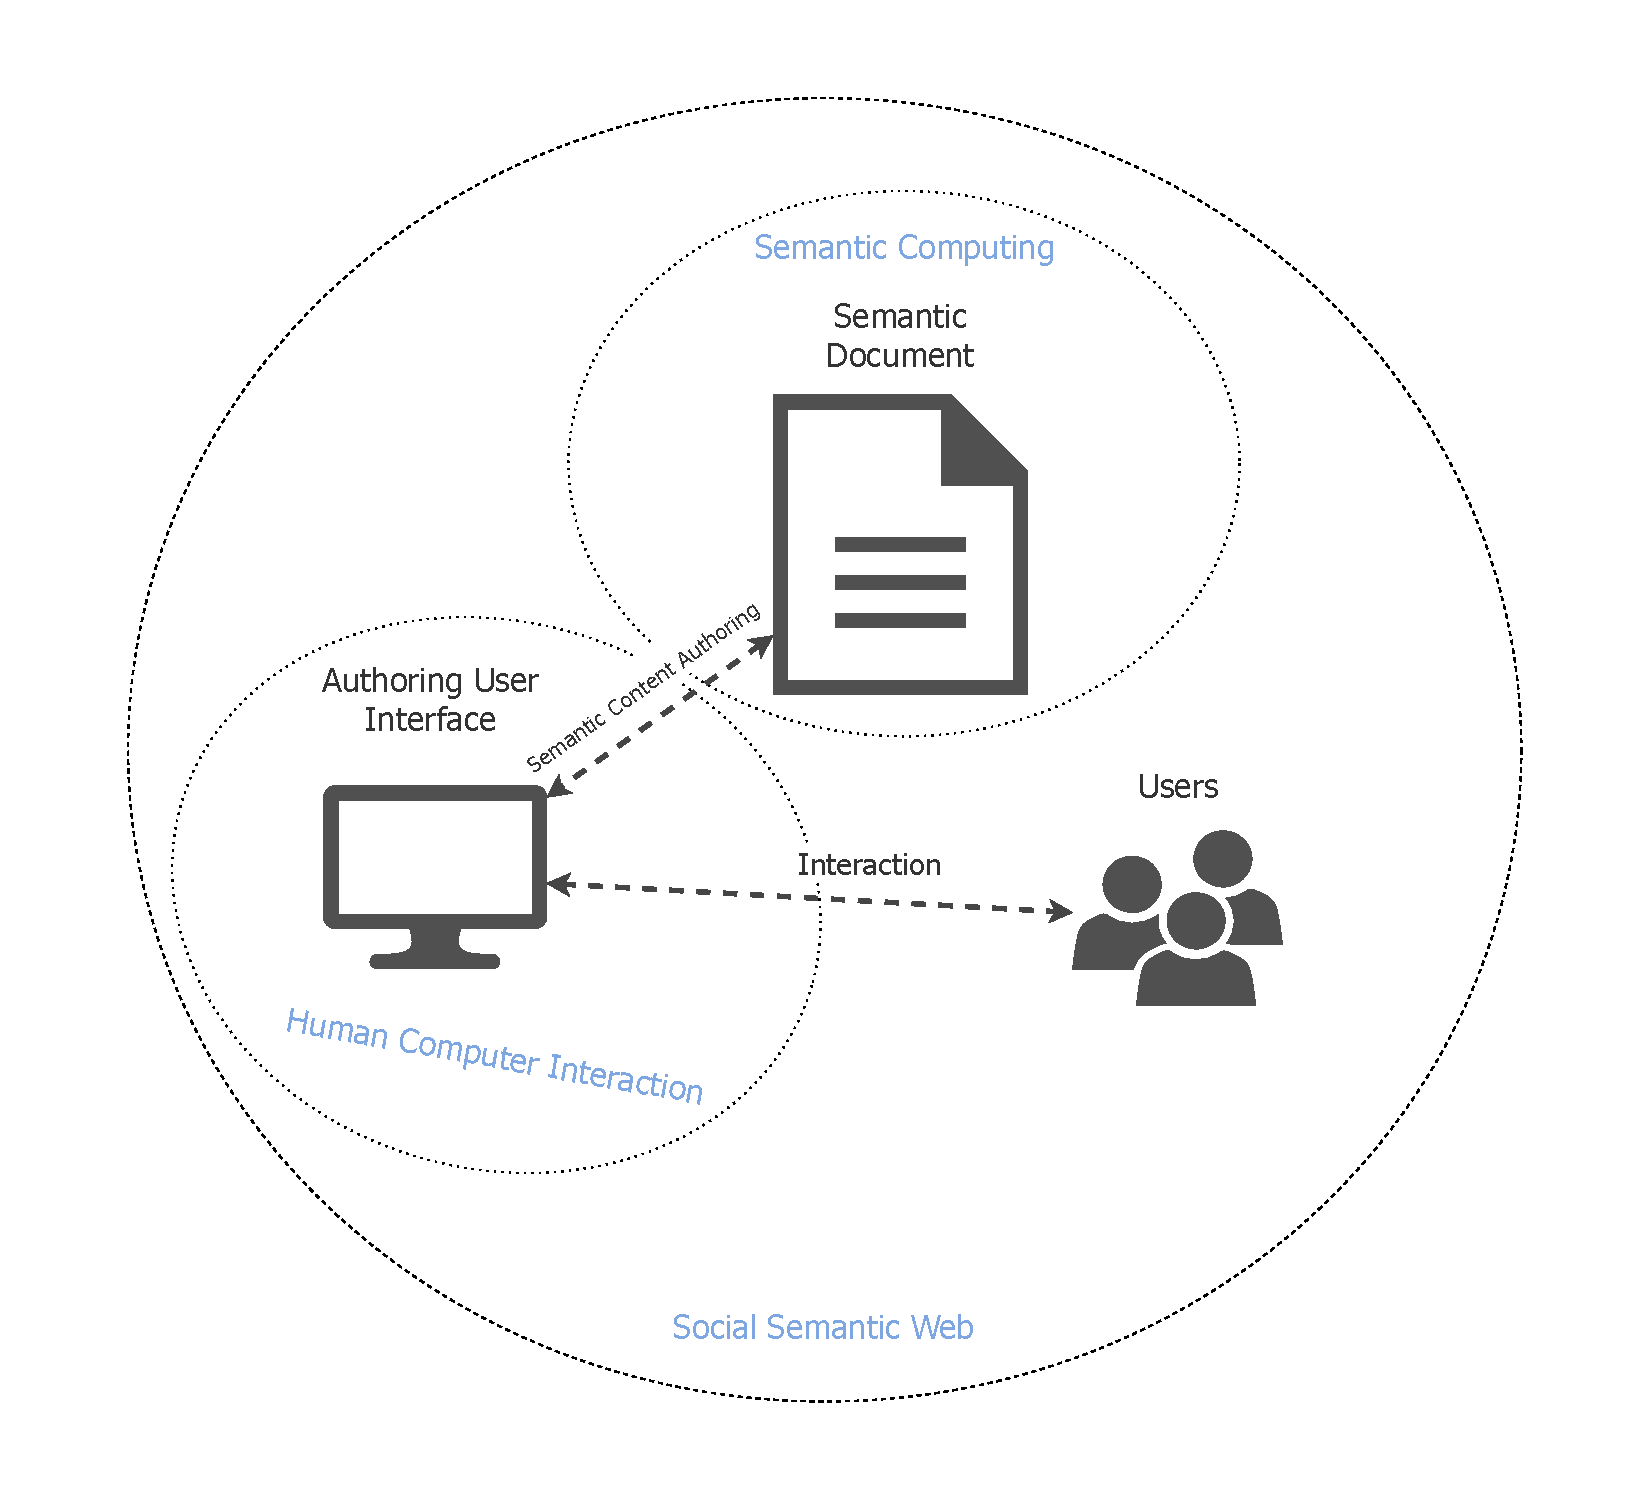
\includegraphics[width=1\textwidth]{drawio/authoring_semantic_ecosystem}
	 \caption{The ecosystem for semantic content authoring}\label{fig:authoring_semantic_ecosystem}
\end{figure}
The central entity of the semantic ecosystem is a semantic document which holds semantically enriched information. 
In information management, semantic documents serve a number of purposes such as information searching, information retrieval, information presentation, information integration, personalisation, reusability and interoperability~\cite{khalili2013}. For that reason there exists a research area dealing with the main fields of semantic content management. In particular, it covers the manipulation, creation and processing of semantic content. Users do not directly interact with semantic documents, but rather through a uniform \gls{ui}. A number of quality attributes for the assessment of \gls{ui}-features of \gls{sca}-Systems were invented~\cite{khalili2013}. The goal was to improve usability, a measure of the effectiveness, efficiency and satisfaction a user achieves. 

A number of tools for semantic content authoring were developed. A prominent example is OntoWiki~\cite{auer2006}, an open-source Semantic Wiki originally focusing on collaboration but evolved as an ontology editor and platform for knowledge acquisition. It was inspired by other Wiki systems but primarily focusing on managing \gls{rdf} knowledge bases.  Another tool, adding Crowdsourcing capabilities to ontology development activities is Mechanical~Protege\footnote{\url{http://people.aifb.kit.edu/yt2652/mechanicalProtege/}}. The tool is actually a plug-in for the ontology editor Protege\footnote{\url{https://protege.stanford.edu/} accessed 2018/08/07}. 

\paragraph{Data Linking}
The next principle according to the Linked Data Life-Cycle is the Data Linking principle. It is by far the most important principle because it 
underlines the distributed nature of Linked Data. Instead of the traditional definition of data where information is stored in silos with little or no 
relations to the outside, Linked Data sources are distributed, containing many links to other data sources. This paradigm perfectly fits into the distributed nature of the Web, turning it into a source of distributed information optimised for querying and browsing. 

\paragraph{Classification and Enrichment}
Over time, Linked Data sources grow in size and expressiveness. This principle refers to the process of extending the expressiveness and richness 
of semantic knowledge bases. It means that instead of creating the structure upfront, the knowledge base evolves over time. For that, the knowledge 
base is typically enriched by analysing existing data to improve or extend its schema. A variety of (semi-)~automatic enrichment approaches emerged over the past years. The methods span across several research areas, including machine learning, statistics, natural language processing, to name just a few. 

\paragraph{Data Analysis and Quality}
Due to the distributed nature of Linked Data where information originating from heterogeneous data sources is merged, the quality of the resulting
dataset is often varying. Therefore, a key factor for the adoption of Linked Data is ensuring its quality by identifying and fixing common problems. Before that, it is necessary to determine the quality of the existing dataset. For that, metrics which measure the quality in terms of accuracy, completeness, adequacy and degree of understandability need to be defined. \cite{zaveri2016} defines useful quality metrics along with 26 quality dimensions that help to measure the quality of the Linked Data.

\paragraph{Data Cleansing and Evolution}
After the quality is analysed and problems are detected, strategies for fixing these problems are needed. In constantly evolving datasets with millions or even billions of \gls{rdf} triples it is important to keep the links between datasets. Likewise, conflicts and discrepancies in datasets can cause real trouble. Repairing such inconsistencies in overlapping datasets is called \emph{Data Fusion}. Several works focusing on repairing problematic datasets appeared in the literature. For example, \cite{mendes2012} considers repairing with respect to data fusion and \cite{flouris2012} investigates how provenance helps to improve the quality of Linked Data. In this context, provenance refers to where and how the data was obtained from. 

\paragraph{Data Browsing and Querying}
Last, users have the opportunity to explore the Linked Data available on the Web in a fast and efficient way. A prominent way to query Linked Data is
\gls{sparql}\footnote{\url{https://www.w3.org/TR/rdf-sparql-query/} accessed 2019/01/17}, a query language specifically designed to retrieve and manipulate Linked Data. There are similarities between \gls{sql} and \gls{sparql} in terms of query structure, but there are also differences.